\documentclass[12pt]{article}
\usepackage[english]{babel}
\usepackage[utf8x]{inputenc}
\usepackage{amsmath}
\usepackage{tikz}
\usetikzlibrary{arrows,automata}
\begin{document}

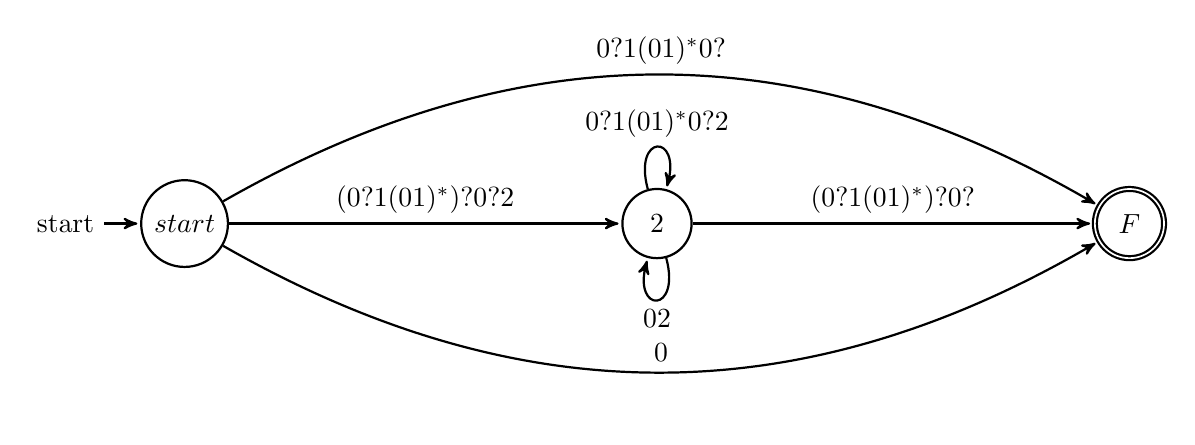
\begin{tikzpicture}[->,>=stealth',shorten >=1pt,auto,node distance=6cm,
    thick,base node/.style={circle,draw,minimum size=8pt}, real node/.style={double,circle,draw,minimum size=17pt}]

  \node[state,initial] (start) {$start$};
 
  \node[state] (2) [right of=start] {$2$};
  \node[state,accepting] (F) [right of=2] {$F$};
  
  \path 
        (start) edge [bend right] node {$0$} (F)
        (start) edge [bend left] node {$0?1(01)^{*}0?$} (F)
        (start) edge  node {$(0?1(01)^{*})?0?2$} (2)
        (2)
         edge   node {$(0?1(01)^{*})?0?$} (F)
         edge [loop below] node {$02$} ( )
         edge [loop above] node {$0?1(01)^{*}0?2$} ( )
         ;

\end{tikzpicture}
\end{document}https://www.overleaf.com/project/5f66c6dd8387d300018234e8